%%%%%%%%%%%%%%%%%%%%%%%%%%%%%%%%%%%%%%%%%
% Short Sectioned Assignment
% LaTeX Template
% Version 1.0 (5/5/12)
%
% This template has been downloaded from:
% http://www.LaTeXTemplates.com
%
% Original author:
% Frits Wenneker (http://www.howtotex.com)
%
% License:
% CC BY-NC-SA 3.0 (http://creativecommons.org/licenses/by-nc-sa/3.0/)
%
%%%%%%%%%%%%%%%%%%%%%%%%%%%%%%%%%%%%%%%%%

%----------------------------------------------------------------------------------------
%	PACKAGES AND OTHER DOCUMENT CONFIGURATIONS
%----------------------------------------------------------------------------------------

\documentclass[paper=a4, fontsize=11pt]{scrartcl} % A4 paper and 11pt font size

\usepackage[T1]{fontenc} % Use 8-bit encoding that has 256 glyphs
\usepackage{fourier} % Use the Adobe Utopia font for the document - comment this line to return to the LaTeX default
\usepackage[english]{babel} % English language/hyphenation
\usepackage{amsmath,amsfonts,amsthm} % Math packages
\usepackage{csvsimple}
\usepackage{graphicx}

\usepackage{sectsty} % Allows customizing section commands
\allsectionsfont{\centering \normalfont\scshape} % Make all sections centered, the default font and small caps

\usepackage{fancyhdr} % Custom headers and footers
\pagestyle{fancyplain} % Makes all pages in the document conform to the custom headers and footers
\fancyhead{} % No page header - if you want one, create it in the same way as the footers below
\fancyfoot[L]{} % Empty left footer
\fancyfoot[C]{} % Empty center footer
\fancyfoot[R]{\thepage} % Page numbering for right footer
\renewcommand{\headrulewidth}{0pt} % Remove header underlines
\renewcommand{\footrulewidth}{0pt} % Remove footer underlines
\setlength{\headheight}{13.6pt} % Customize the height of the header

\numberwithin{equation}{section} % Number equations within sections (i.e. 1.1, 1.2, 2.1, 2.2 instead of 1, 2, 3, 4)
\numberwithin{figure}{section} % Number figures within sections (i.e. 1.1, 1.2, 2.1, 2.2 instead of 1, 2, 3, 4)
\numberwithin{table}{section} % Number tables within sections (i.e. 1.1, 1.2, 2.1, 2.2 instead of 1, 2, 3, 4)

\setlength\parindent{0pt} % Removes all indentation from paragraphs - comment this line for an assignment with lots of text

%----------------------------------------------------------------------------------------
%	TITLE SECTION
%----------------------------------------------------------------------------------------

\newcommand{\horrule}[1]{\rule{\linewidth}{#1}} % Create horizontal rule command with 1 argument of height

\title{	
\normalfont \normalsize 
%\textsc{university, school or department name} \\ [25pt] % Your university, school and/or department name(s)
\horrule{0.5pt} \\[0.4cm] % Thin top horizontal rule
\huge Handin 1 \\ % The assignment title
\horrule{2pt} \\[0.5cm] % Thick bottom horizontal rule
}

\author{S\o ren Meldgaard 201303712, Malthe Bisbo 201303718} % Your name

\date{\normalsize\today} % Today's date or a custom date

\begin{document}

\maketitle % Print the title

\section{Status of work}
The model worked well with AC values between 0.3 and 0.45 in the test set.
\section{Model structure}

In order to translate the annotations into sequences of hidden states, we have used the following strategy.
All the annotations start with an N, which is immediately translated into the hidden state 0. Then we look at the next 4 annotations. If we encounter 'NCCC' we look in the genome file and assign '0XYZ' where 'XYZ' is the corresponding start-code. If we do not recognize the start-code we simply label the next coding part as non-coding. If we have encountered a start-code we then look for 'CCC' and label it '[10, 11, 12]' until we find one of the three stop-codes. After looking for 'NCCC' we look for 'NRRR' and the procceed in the same way as for 'NCCC'. If none of the two have been found it must be an 'N' which we then label as '0'. The process is then repeated for the next base. This means that we would miss 'RRRCCC', since we look for 'NCCC' and then 'NRRR', but we have assumed that it has neglible effect.

\section{Gene prediction}
In order to predict the gene structures for the sequences without annotation we have trained our model by counting. Then the Viterbi-algorithm is used to decode the sequence (X) provinding a sequence of hidden states (Z). This is then easily translated into an annotation, since hidden state '0' corresponds to 'N', 1 to 21 is 'C' and 22 to 42 is 'R'.

\section{Performance of gene predictor}
In order to train the model 5 genomes with known annotations are available. To check the performance the HMM is trained on 4 of them and then used to predict the one left out. This prediction is then compared to the correction annotation. This is done for all five permutations, with the results for each stage of cross validation shown below. \\

\textbf{Validating on genome1:} \\
Cs   (tp=658123, fp=166731, tn=301163, fn=58582): Sn = 0.9183, Sp = 0.7979, AC = 0.5985 \\
Rs   (tp=546592, fp=121250, tn=306046, fn=53699): Sn = 0.9105, Sp = 0.8184, AC = 0.6480 \\
Both (tp=1204715, fp=287981, tn=247464, fn=112281): Sn = 0.9147, Sp = 0.8071, AC = 0.4359 \\

\textbf{Validating on genome2:} \\
Cs   (tp=756778, fp=154730, tn=307365, fn=57869): Sn = 0.9290, Sp = 0.8302, AC = 0.6330 \\
Rs   (tp=796436, fp=138307, tn=305126, fn=60108): Sn = 0.9298, Sp = 0.8520, AC = 0.6527 \\
Both (tp=1553214, fp=293037, tn=247257, fn=117977): Sn = 0.9294, Sp = 0.8413, AC = 0.4527 \\


\textbf{Validating on genome3:} \\
Cs   (tp=928852, fp=142151, tn=442271, fn=110668): Sn = 0.8935, Sp = 0.8673, AC = 0.6587
Rs   (tp=824584, fp=236489, tn=472544, fn=80395): Sn = 0.9112, Sp = 0.7771, AC = 0.6047
Both (tp=1753436, fp=378640, tn=361876, fn=191063): Sn = 0.9017, Sp = 0.8224, AC = 0.4336

\textbf{Validating on genome4:} \\
Cs   (tp=590520, fp=139488, tn=331346, fn=66225): Sn = 0.8992, Sp = 0.8089, AC = 0.6226
Rs   (tp=545012, fp=124255, tn=317385, fn=80186): Sn = 0.8717, Sp = 0.8143, AC = 0.6015
Both (tp=1135532, fp=263743, tn=251160, fn=146411): Sn = 0.8858, Sp = 0.8115, AC = 0.4084

\textbf{Validating on genome5:} \\
Cs   (tp=928852, fp=142151, tn=442271, fn=110668): Sn = 0.8935, Sp = 0.8673, AC = 0.6587 \\
Rs   (tp=824584, fp=236489, tn=472544, fn=80395): Sn = 0.9112, Sp = 0.7771, AC = 0.6047 \\
Both (tp=1753436, fp=378640, tn=361876, fn=191063): Sn = 0.9017, Sp = 0.8224, AC = 0.4336 \\

\section{Model used on unknown structures}
Finally the model is trained on all 5 known genomes and then used to predict 5 unknown genomes. The results are seen below. 

\textbf{Genome 6} \\
Cs   (tp=757705, fp=162923, tn=305888, fn=56493): Sn = 0.9306, Sp = 0.8230, AC = 0.6251 \\
Rs   (tp=717157, fp=127673, tn=305405, fn=56976): Sn = 0.9264, Sp = 0.8489, AC = 0.6616 \\
Both (tp=1474862, fp=290596, tn=248912, fn=113469): Sn = 0.9286, Sp = 0.8354, AC = 0.4561 \\

\textbf{Genome 7} \\
Cs   (tp=869896, fp=235340, tn=517864, fn=78584): Sn = 0.9171, Sp = 0.7871, AC = 0.6300 \\
Rs   (tp=814804, fp=226043, tn=512895, fn=83553): Sn = 0.9070, Sp = 0.7828, AC = 0.6219 \\
Both (tp=1684700, fp=461383, tn=434311, fn=162137): Sn = 0.9122, Sp = 0.7850, AC = 0.4551 \\

\textbf{Genome 8} \\
Cs   (tp=708076, fp=137639, tn=350466, fn=73033): Sn = 0.9065, Sp = 0.8373, AC = 0.6447 \\
Rs   (tp=607901, fp=169000, tn=349048, fn=74451): Sn = 0.8909, Sp = 0.7825, AC = 0.5857 \\
Both (tp=1315977, fp=306639, tn=276015, fn=147484): Sn = 0.8992, Sp = 0.8110, AC = 0.4179 \\

\textbf{Genome 9}\\
Cs   (tp=779967, fp=205635, tn=339297, fn=86130): Sn = 0.9006, Sp = 0.7914, AC = 0.5561 \\
Rs   (tp=759252, fp=218154, tn=332691, fn=92736): Sn = 0.8912, Sp = 0.7768, AC = 0.5270 \\
Both (tp=1539219, fp=423789, tn=246561, fn=178866): Sn = 0.8959, Sp = 0.7841, AC = 0.3137 \\

\textbf{Genome 10} \\
Cs   (tp=613866, fp=108336, tn=251583, fn=87402): Sn = 0.8754, Sp = 0.8500, AC = 0.5833 \\
Rs   (tp=371956, fp=137342, tn=288785, fn=50200): Sn = 0.8811, Sp = 0.7303, AC = 0.5705 \\
Both (tp=985822, fp=245678, tn=201383, fn=137602): Sn = 0.8775, Sp = 0.8005, AC = 0.3613 \\

% Example of figure
%\begin{figure}[h]
%\center
%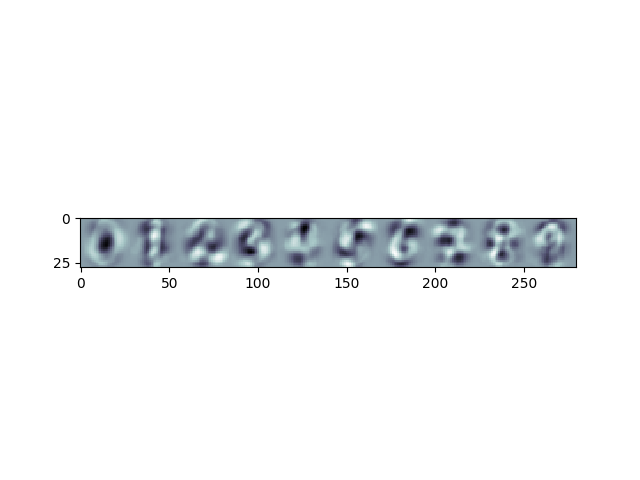
\includegraphics[trim={0 4.5cm 0 5cm},clip]{logistic_regression_parameter_plot_1_128.png}
%\end{figure}

% Example of csv table
% \csvautotabular{softmax_confusion_matrix.csv} \\ \\ \\

\begin{figure*}
	\centering
	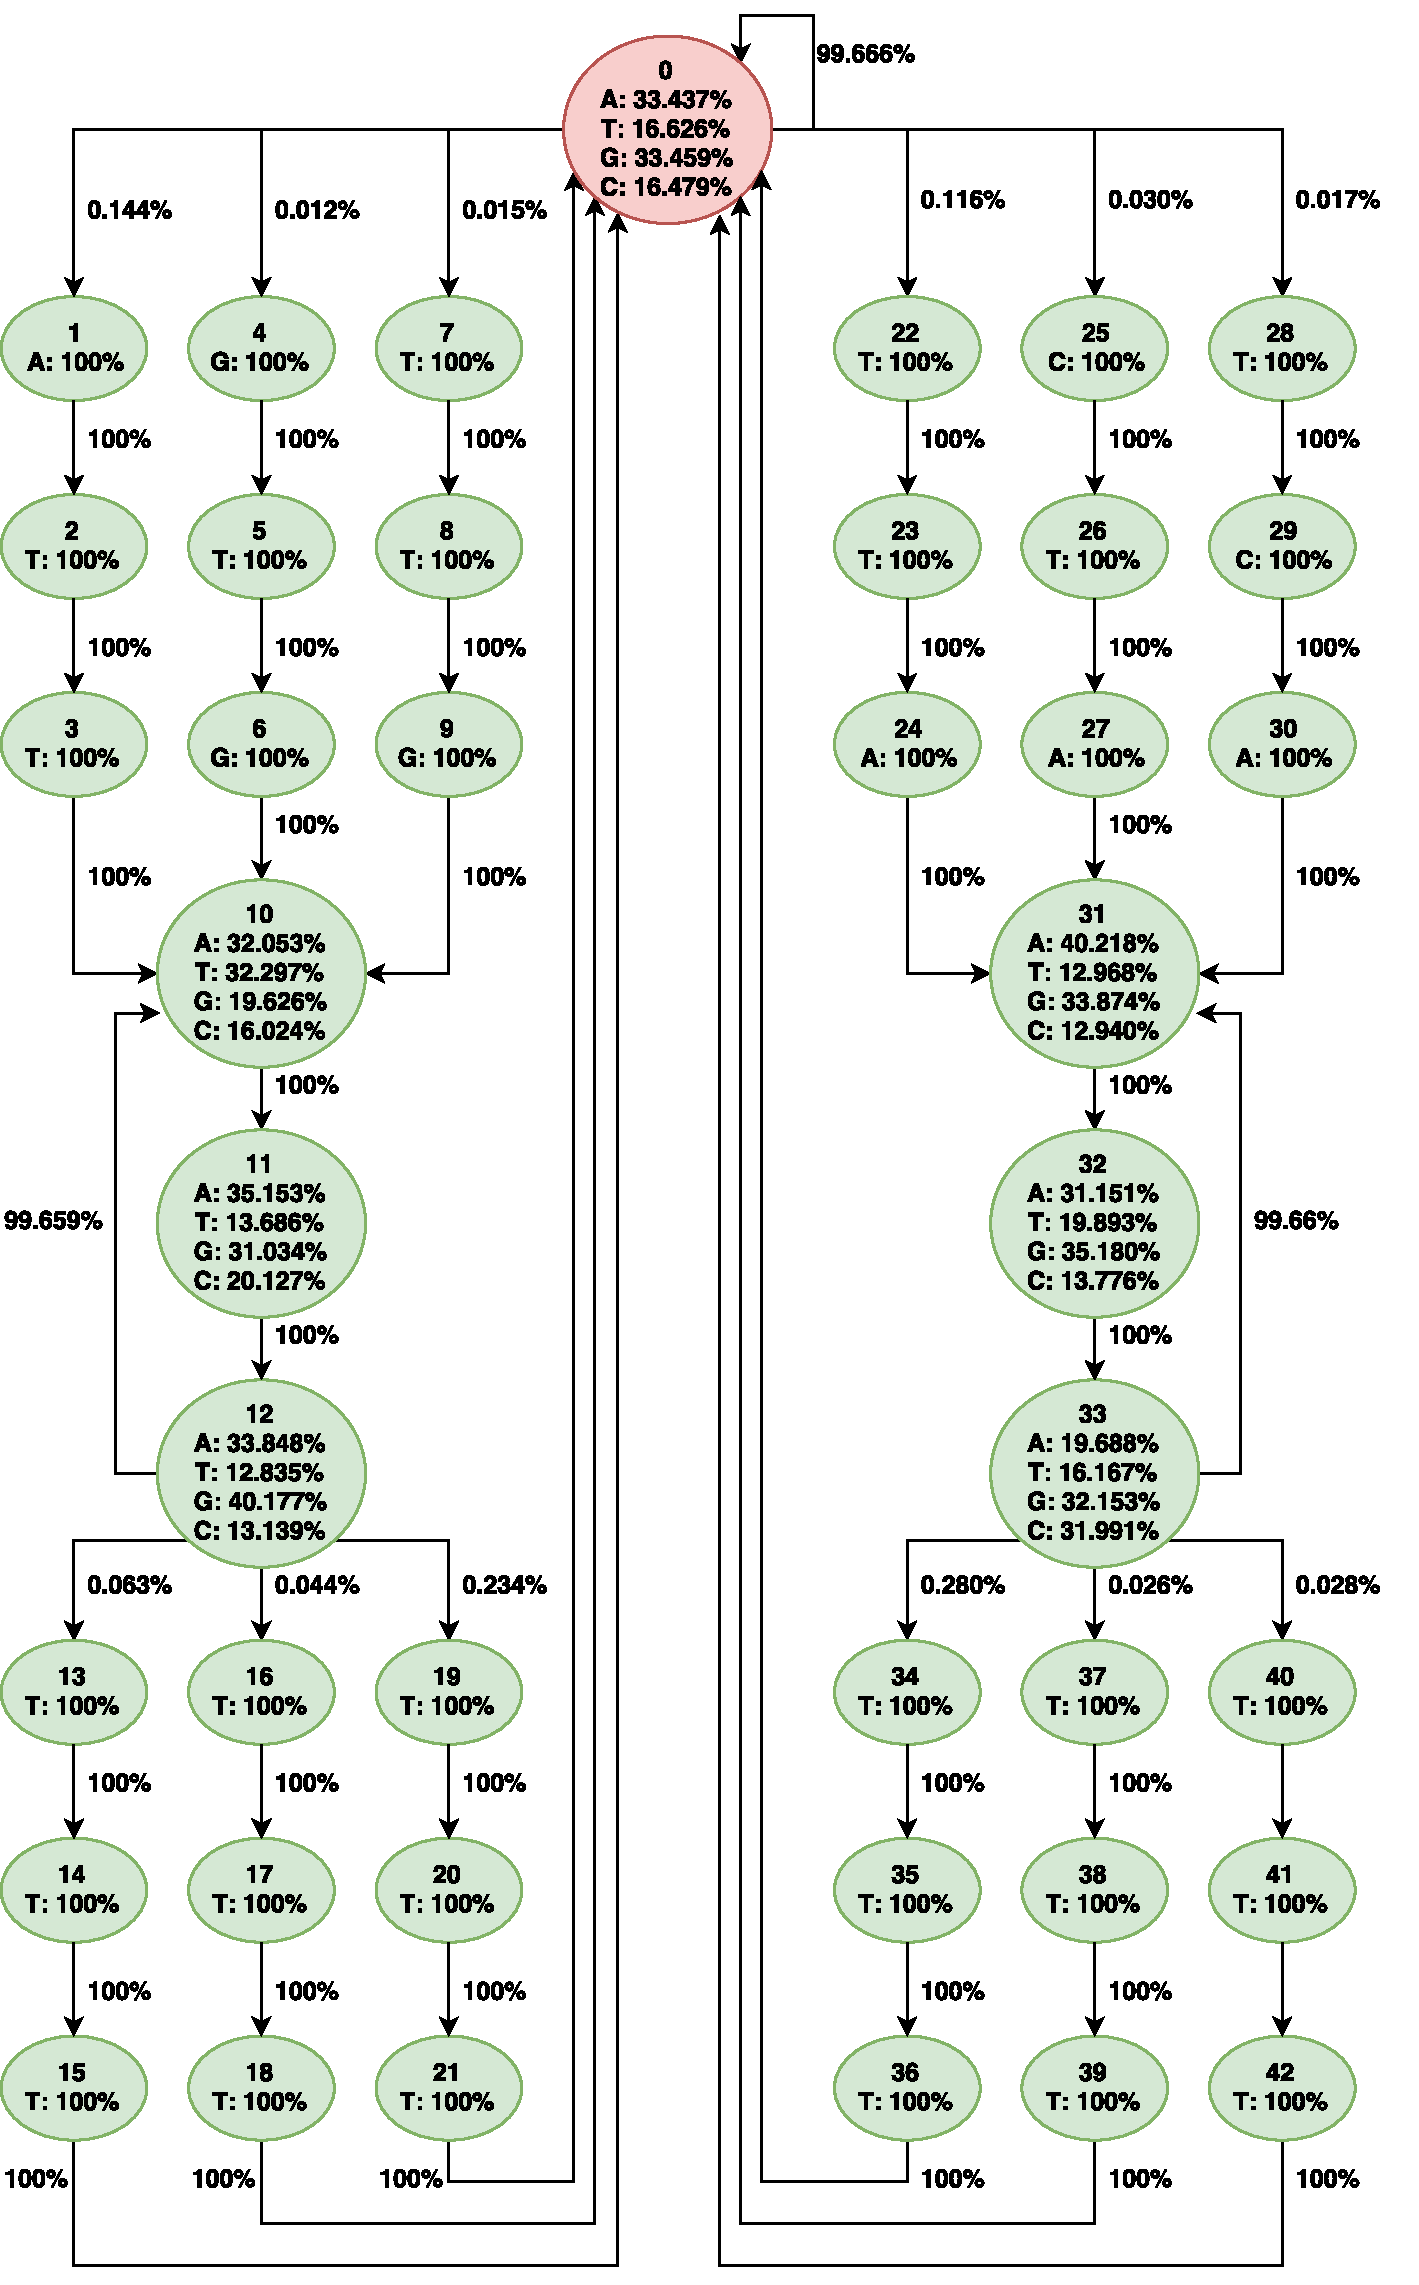
\includegraphics[width=0.9\linewidth]{43state_model}
	\caption{}
	\label{fig:43statemodel}
\end{figure*}

\end{document}